%!TEX root = ../fys_cursus.tex

%\the\textwidth
% 390 pt = 13.7323943 cm (1pt=28,4 cm)

\chapter{Golven}

Als je een steentje in een poel gooit, krijg je van die prachtige uitdijende cirkels in het wateroppervlak, die, al naargelang ze groter worden, ook in zichtbaarheid afnemen en meer en meer verdwijnen. De verstoring die door de steen in het wateroppervlak teweeg is gebracht, plant zich voort in het water. We hebben te maken met een golf.
\newline
Een bijzondere eigenschap van de golf die in het wateroppervlak ontstaat is dat het de verstoring in het medium is die zich verplaatst, niet het water zelf. Het water blijft ter plaatse. Zo zal een dobber van een vislijn enkel op en neer bewegen wanneer een golf voorbijkomt. Ook bij een Mexican wave is dit duidelijk; het zijn niet de supporters die rondlopen!
\newline
Golven hebben echter niet altijd een medium nodig om zich in voort te planten. Denk maar aan licht of in het algemeen aan een elektromagnetische golf. De wisselende elektrische en magnetische velden vormen hier de golf.

%een golf heeft een trilling als bron. Als de bron een harmonische trilling uitvoert, ontstaat een golf die zowel in de ruimte als in de tijd sinuso\"idaal is.

%golf = def

\section{Golven \& kenmerken}

Golven kunnen we volgens hun kenmerken indelen in een paar categori\"en. Zo kunnen we een onderscheid maken tussen \emph{mechanische} en \emph{elektromagnetische} golven. Mechanische golven hebben een (elastisch\footnote{De vervorming in het medium kan zich maar voortzetten van zodra het lichaam te vervormen is en dus elastisch is. Er moeten immers krachten tussen de verschillende plaatsen van het medium aanwezig zijn.}) medium nodig om zich in te verplaatsen -- het is de storing in het medium die de golf vormt. Elektromagnetische golven daarentegen hebben geen medium nodig. Het zijn de elektrische en de magnetische veldenvectoren die golven.\footnote{Ook de recentelijk gemeten zwaartekrachtgolven moeten tot de categorie behoren van golven die geen medium nodig hebben. Het zijn rimpelingen van de ruimte-tijd zelf.}
\begin{figure}[h]
\centering
\includegraphics[width=0.7\textwidth]{elasticiteit_medium}
\caption{\textit{Een golfpuls die zich voortplant in een touw. De pijlen geven de snelheid van deeltjes in het touw weer.}}
\end{figure}
\newline
\newline
Golven kunnen \emph{transversaal} of \emph{longitudinaal} zijn. Bij een transversale golf gebeurt de beweging van de deeltjes van het medium loodrecht op de voortplantingsrichting van de golf. Zo krijg je transversale golven wanneer je het uiteinde van een touw heen en weer slingert. Ook licht is een transversale golf. Hier trilt dus niet het medium maar is het de ori\"entatie van de elektrische of magnetische veldvector die loodrecht staat op de voortplantingsrichting. Bij een longitudinale golf bewegen de deeltjes van het medium in de richting evenwijdig met de voortplantingsrichting. P-golven bij een aardbeving zijn hiervan een voorbeeld (i.t.t. S-golven, die zijn transversaal). Ook geluid bestaat uit een longitudinale golf. Zo plant geluid zich in de lucht voort doordat de luchtmoleculen tegen elkaar botsen. 
Er zijn nog andere soorten golven zoals \emph{oppervlaktegolven}, \emph{tweedimensionale} en \emph{driedimensionale} golven. Deze zullen we hier met momenten kort behandelen.
\begin{figure}[h]
\centering
\includegraphics[width=0.9\textwidth]{longitudinaal_veer}
\caption{\textit{Een longitudinale golf in een opgegespannen veer. De verplaatsingen van de spiralen zijn in de richting van de zich voortplantende golf. Elke samendrukking wordt gevolgd door een uitrekking.}}
\end{figure}
\newline
\newline
Als een de bron van een golf voortdurend blijft trillen, spreken we van een \emph{continue golf} of lopende golf. Als je slechts een enkele verstoring hebt die zich voortplant, spreken we van een \emph{puls}. We zullen hier in de regel over continue golven spreken.
\newline
\newline
Om een golf te kunnen beschrijven, hebben we een paar karakteristieke grootheden. Zo kunnen we bij een continue golf spreken over de \emph{golflengte}. De golflengte $\lambda$ van een golf is de kortste afstand tussen twee punten die in fase trillen. Deze is gemakkelijk terug te vinden als de afstand van top tot top\footnote{In de ruimtelijke voorstelling van de golf kan je over golftoppen, -pieken of -kammen spreken tegenover golfdalen. Voor een longitudinale golf spreken we over samendrukkingen of verdichtingen versus uitrekkingen of verdunningen.}. De golflengte is dus de periode voor de golf in de ruimte zoals de `periode' $T$ de periode is van een trilling in de tijd. Voor een continue golf is de \emph{periode} de tijd die een deeltje nodig heeft om een volledige trilling te doorlopen. Omdat dit evenzeer de tijd is die de storing nodig heeft om de golflengte af te leggen, hebben we de volgende eenvoudige maar belangrijke formule voor de snelheid waarmee de golf zich voortplant -- de \emph{golfsnelheid} of fasesnelheid:
\begin{equation*}
v=\frac{\lambda}{T}=\lambda\cdot f
\end{equation*}
%De eenheid van golflengte is dan ook de meter, daar waar die voor de periode de seconde is.
In de regel zullen we golven behandelen waarvoor de snelheid onafhankelijk is van de frequentie of golflente van de golf.\footnote{Is de snelheid wel afhankelijk van de frequentie, dan spreken we over dispersie. Dit verschijnsel doet zich onder andere voor bij licht dat door een prisma gaat. De snelheid voor verschillende kleuren en dus frequenties is verschillend waardoor je een regenboogeffect krijgt. De snelheid bepaalt immers de mate van breking.} In dat geval zijn golflengte en frequentie dus omgekeerd evenredig.
\newline
\newline
Voor een golf kan je naast de golfsnelheid nog een andere snelheid beschouwen. De deeltjes van het medium kunnen namelijk harmonisch trillen zodat hun snelheidsverloop helemaal verschillend is van de constante golfsnelheid waarmee de storing zich voortplant. De onderstaande figuur verduidelijkt dit.
\begin{figure}[h]
\centering
\includegraphics[width=0.9\textwidth]{golf_vs_deeltjessnelheid}
\caption{\textit{De golf beweegt naar rechts terwijl de deeltjes van het touw oscilleren.}}
\end{figure}

%- overdracht van energie

\section{Periodieke golven}

Zoals we de positie van een voorwerp konden beschrijven met een functie $x(t)$, willen we ook een golf m.b.v. een functie kunnen beschrijven. Omdat een golf niet te lokaliseren is in een punt maar zich uitstrekt over de hele ruimte en daarnaast in de tijd evolueert, hebben we een iets uitgebreidere functie nodig. De uitwijking $y$ van het medium is zowel afhankelijk van de plaats $x$ waarop je kijkt als het moment $t$ dat je interesseert. De oplossing bestaat erin een functie in twee variabelen te gebruiken. 
\newline
\newline
We beschouwen een sinuso\"idale golf die naar rechts beweegt -- volgens de $x$-as. Om een wiskundige beschrijving van een golf te vinden, bekijken we twee momentopnames op willekeurige tijdstippen. Voor het gemak nemen we als eerste tijdstip $t=0$ en noemen we het tweede tijdstip $t$. In de tijdsspanne $t$ is de golf $vt$ eenheden naar rechts opgeschoven, zie figuur (\ref{afleiding_golfvergelijking}). $v$ is uiteraard de golfsnelheid.

\begin{figure}[!h]
\centering

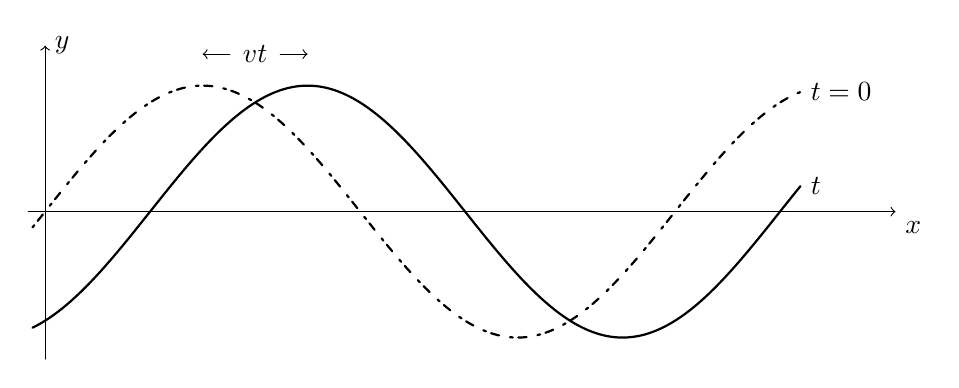
\begin{tikzpicture}[line cap=round,line join=round,x=8.0cm,y=8.0cm]
%\draw[very thin,color=gray] (0,-0.24) grid (1.4,0.24);
\draw[->,color=black] (-0.026820246306000255,0.) -- (1.35,0) node [anchor=north west] { $x$};
%\foreach \x in {0.1,0.2,0.3,0.4,0.5,0.6,0.7,0.8,0.9,1.,1.1,1.2,1.3,1.4}
%\draw[shift={(\x,0)},color=black] (0pt,2pt) -- (0pt,-2pt);
%\draw[color=black] (1.4,0) node [anchor=north west] { $x$};
\draw[->,color=black] (0.,-0.2341604564505571) -- (0.,0.2636169400770265) node [anchor=west] { $y$};
%\foreach \y in {-0.2,-0.1,0.1,0.2}
%\draw[shift={(0,\y)},color=black] (2pt,0pt) -- (-2pt,0pt);
%\draw[color=black] (0.008952830872798266,0.22422448423671415) node [anchor = south west] { $y$};
%\clip(-0.026820246306000255,-0.2341604564505571) rectangle (1.464721377102191,0.2636169400770265);
\draw[line width=0.8pt,dash pattern=on 1pt off 2pt on 3pt off 4pt,smooth,samples=100,domain=-0.02:1.2] plot(\x,{0.2*sin((6.283185307179586*(\x)-6.283185307179586)*180/pi)}) node[right] {$t=0$};
\draw[line width=0.8pt,smooth,samples=100,domain=-0.02:1.2] plot(\x,{0.2*sin((6.283185307179586*(\x)-6.283185307179586*(1.0+1/6))*180/pi)}) node[right] {$t$};
%\draw (0.03943070215270692,2.6289548566703287) node[anchor= north west] {$y$};
\draw[<-] (2/8,2/8) -- (2/8+1/12-0.04,2/8);
\draw[->] (2/8+1/12+0.04,2/8) -- (2/8+1/6,2/8);
\draw (1/3,2/8) node {$vt$};
\end{tikzpicture}

\caption{\emph{De uitwijking van een golf in functie van de tijd op $t=0$ en een willekeurig tijdstip $t$}}\label{afleiding_golfvergelijking}
\end{figure}

De verschijningsvorm van de golf in de ruimte kunnen we op $t=0$ weergeven met volgende sinusfunctie:
\begin{eqnarray*}
y=A\sin(kx)\qquad\mathrm{met}\qquad k=\frac{2\pi}{\lambda}
\end{eqnarray*}
Het symbool $k$ noemen we het \emph{golfgetal}.\footnote{De $k$ is eigenlijk niets anders dan de `$b$' zoals je die kent in de algemene sinusfunctie $f(x)=a\sin(b(x-c))$+d. $b=\frac{2\pi}{p}$ met $p$ de periode. In deze context is de periode de golflengte $\lambda$, uitgedrukt in meters.} \footnote{De $k$ heeft niets te maken met de veerconstante. Het is niet omdat Jantje Jantje heet en Jantje Jantje, dat Jantje en Jantje dezelfde personen zijn. Jantje en Jantje kunnen bijvoorbeeld -- al is het onwaarschijnlijk -- broers zijn.}
\newline
\newline
Een tijd $t$ later is de verschijningsvorm van de golf een afstand $vt$ (de afstand die een top gedurende de tijd $t$ heeft afgelegd) naar rechts opgeschoven. De vergelijking vinden we dan door een overeenkomstige verschuiving door te voeren:
\begin{eqnarray*}
y&=&A\sin(k(x-vt))\\
%&=&A\sin(kx-kvt)\\
&=&A\sin\left(kx-\frac{2\pi v}{\lambda}t\right)\\
&=&A\sin\left(kx-\frac{2\pi}{T}t\right)\\
&=&A\sin\left(kx-\omega t\right)
\end{eqnarray*}
We hebben de uitwijking $y$ kunnen schrijven in functie van de variabelen $x$ en $t$. We hebben een algemene uitdrukking voor een rechtslopende golf:
\begin{eqnarray}
y(x,t)&=&A\sin\left(kx-\omega t\right)\label{rechtslopende_golf}
\end{eqnarray}
Om de vergelijking voor een linkslopende golf te vinden, verschuiven we naar links in plaats van naar rechts of vervangen we $v$ door $-v$. We krijgen dan
\begin{eqnarray}
y(x,t)&=&A\sin\left(kx+\omega t\right)\label{linkslopende_golf}
\end{eqnarray}
Deze functie in twee variabelen kunnen we iets beter verstaan wanneer we \'e\'en van de variabelen constant houden en de afhankelijkheid van de overblijvende variabele bekijken. Zo hebben we, wanneer we op een vaste plaats $x=x_0$ kijken, een harmonische trilling:
\begin{eqnarray*}
y_{x_0}(t)&=&y(x_0,t)=A\sin(\omega t+\underbrace{kx_0}_{\rm beginfase})
\end{eqnarray*}
Het is als het ware een patrijspoort van een stilstaand schip ter hoogte van de waterlijn. Een voorbijkomende golf is door het kleine venstertje slechts waar te nemen door het op- en neergaan van het waterniveau. Als we de tijd vastleggen door te kijken op \'e\'en bepaald tijdstip $t=t_0$, hebben we een functie die enkel de golf in de ruimte beschrijft.
\begin{eqnarray*}
y_{t_0}(x)&=&y(x,t_0)=A\sin(kx+\omega t_0)
\end{eqnarray*}
Het is alsof we een foto trekken van de golf.


\newpage

%\section{Verschijnselen}
%
%%\includepdf[pages={1},scale=1]{./golven_giancoli/scan_0.pdf}
%
%\begin{figure}[h]
%\flushright
%\includegraphics[width=0.8\textwidth]{./golven_giancoli/scan_0}
%\end{figure}
%
%\begin{figure}[h]
%\centering
%\includegraphics[width=1.1\textwidth]{./golven_giancoli/scan_1}
%\end{figure}
%
%\begin{figure}[h]
%\centering
%\includegraphics[width=1.1\textwidth]{./golven_giancoli/scan_2}
%\end{figure}
%
%\begin{figure}[h]
%\centering
%\includegraphics[width=1.1\textwidth]{./golven_giancoli/scan_3}
%\end{figure}
%
%\begin{figure}[h]
%\centering
%\includegraphics[width=1.1\textwidth]{./golven_giancoli/scan_4}
%\end{figure}
%
%\begin{figure}[h]
%\centering
%\includegraphics[width=1.1\textwidth]{./golven_giancoli/scan_5}
%\end{figure}
%
%\begin{figure}[h]
%\centering
%\includegraphics[width=1.1\textwidth]{./golven_giancoli/scan_6}
%\end{figure}
%
%\begin{figure}[h]
%\centering
%\includegraphics[width=1.1\textwidth]{./golven_giancoli/scan_7}
%\end{figure}
%
%\begin{figure}[h]
%\centering
%\includegraphics[width=1.1\textwidth]{./golven_giancoli/scan_8}
%\end{figure}
%
%\begin{figure}[h]
%\centering
%\includegraphics[width=0.8\textwidth]{./golven_giancoli/scan_9}
%\end{figure}
%
%\begin{figure}[h]
%\centering
%\includegraphics[width=0.8\textwidth]{./golven_giancoli/scan_10}
%\end{figure}
%
%\begin{figure}[h]
%\centering
%\includegraphics[width=1.1\textwidth]{./golven_giancoli/scan_11}
%\end{figure}
%
%%\begin{figure}[h]
%%\centering
%%\includegraphics[width=1.1\textwidth]{./golven_giancoli/scan_12}
%%\end{figure}
%
%%\begin{figure}[h]
%%\centering
%%\includegraphics[width=1.1\textwidth]{./golven_giancoli/scan_13}
%%\end{figure}
%
%%\subsection{Reflectie}
%%vb echo, licht op een spiegel, zichtbare objecten
%%
%%\subsection{Breking/Refractie}
%%
%%overgang naar een andere middenstof. vb stok in water
%%
%%\subsection{Buiging/diffractie}
%%om de hoek
%%
%%\subsection{Interferentie}
%%
%%- adhv watergolven/abstract?
%%- twee fases? eerst gemakkelijk en vervolgens wiskundig?
%%
%%\section{Staande golven}
%%
%%\begin{tikzpicture}[domain=0:4] 
%%    \draw[very thin,color=gray] (-0.1,-1.1) grid (3.9,3.9);
%%    \draw[->] (-0.2,0) -- (4.2,0) node[right] {$x$}; 
%%    \draw[->] (0,-1.2) -- (0,4.2) node[above] {$f(x)$};
%%    \draw[color=red]    plot (\x,\x)             node[right] {$f(x) =x$}; 
%%    \draw[color=blue]   plot (\x,{sin(\x r)})    node[right] {$f(x) = \sin x$}; 
%%    \draw[color=orange] plot (\x,{0.05*exp(\x)}) node[right] {$f(x) = \frac{1}{20} \mathrm e^x$};
%%  \end{tikzpicture}

